\chapter{Kravspecifikation}

\begin{longtabu} to \linewidth{@{}l l l X[j]@{}}
    Version &    Dato &    Ansvarlig &    Beskrivelse\\[-1ex]
    \midrule
    1.0		&	23-09-2015 &		Alle	&	Første udkast til Use Cases. I alt 4, hvor en af funktionaliteterne var, at man kunne optage en lydsekvens\\[-1ex]
    1.1		&	29-09-2015	&	Alle	&	Ændring af Use Cases efter møde med Peter. I alt 5, hvor funktionaliteterne kunne dækker over de opstillede krav til projektet. \\[-1ex]
    1.2		&	30-09-2015	&	Alle	&	Små ændring af formuleringerne samt byttet om på UC1 og UC2 og tilføjet en UC6. De ikke-funktionelle krav er blevet tilføjet. Klar til Review\\[-1ex]	 

\label{version_Systemark}
\end{longtabu}


\section{Indledning}
Kravspecifikationen vil gennem seks Use Cases beskrive blodtryksmålerens funktionelle krav. Systemet skal kunne vise et blodtryksignal kontinuert i en graf. Systemet skal udover det kunne kalibrer, nulpunkts justeres samt gemme data i en database. Kravspecifikationen indeholder også en række ikke-funktionelle krav, som er listet op efter (F)URPS+.   


\section{Funktionelle krav}
De funktionelle krav vil nedenstående beskrives ud fra Aktør-kontekstdiagram, aktørbeskrivelse, Use Cases samt Use Case diagram. 

\subsection{Aktør-kontekstdiagram}
\begin{figure}[H]
	\centering
	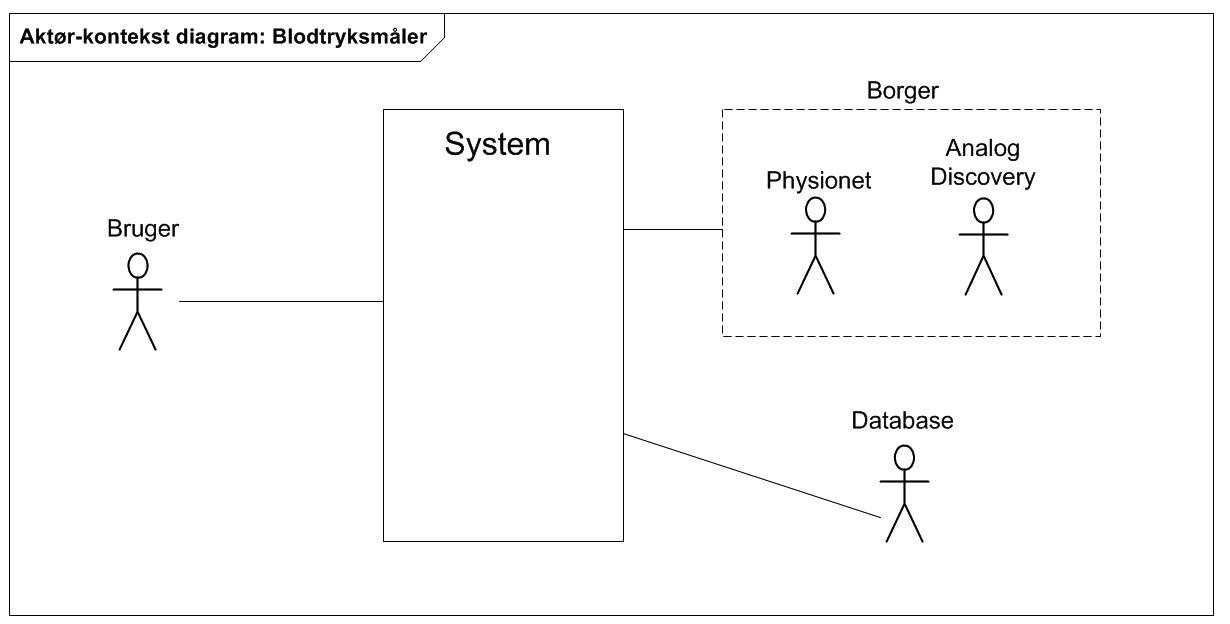
\includegraphics[width=1\textwidth]{Figurer/Snip20150929_7}
	\caption{Aktør-kontekstdiagram}
	\label{fig:aktoerbeskrivelse}
\end{figure}

Systemet består af en software- og en hardward-del. Softwaredelen er udarbejdet i Visual Studio C\#. Hardwaredelen består af flere komponenter sat sammen. Tryktransducer, Instrumentationforstærker, et aktivt 2. ordens lavpasfilter af typen Sallen-Key med unity gain og en DAQ. Det er selve systemet. \\
Primær aktøren i dette projekt er en Bruger. Sekundære aktører er Database og Borger. Borger er en package af Physionet og Analog Discovery, som er eksterne aktører.   

\subsection{Aktørbeskrivelse}

\begin{table}[H]
\begin{tabularx}{\textwidth}{l X}
     Aktørnavn & Bruger \\
     Type & Primær \\
     Beskrivelse  & Person med relevant baggrundsviden inden for blodtryksanalyse \\ 
     \midrule
     Aktørnavn & Borger  \\
     Type & Sekundær \\
     Beskrivelse  & Borger er en kombination af Physionet og Analog Discovery. Borger repræsenterer data fra Physionet leveret til blodtryksmålingssystemet igennem Analog Discovery \\
     \midrule
     Aktørnavn & Database \\
     Type & Sekundær \\
     Beskrivelse  & Database bruges i blodtryksmålingssystemet til at gemme data \\ 
     \midrule
     Atørnavn & Physionet \\
     Type & Ekstern  \\
     Beskrivelse  & Physionet er en ekstern database, som indeholder blodtrykssignalet fra forskellige patienter \\
     \midrule
     Aktørnavn & Analog Discovery  \\
     Type & Ekstern \\
     Beskrivelse  & Analog Discovery omdanner data fra Physionet til at analogt signal \\                                                                                                                                                                          
     \bottomrule                                                                                                                   
    \end{tabularx}
    \caption {Aktørbeskrivelse}
    \label{tab:aktoerbeskrivelse}
	
\end{table}

\subsection{Use case-diagram}
\begin{figure}[H]
	\centering
	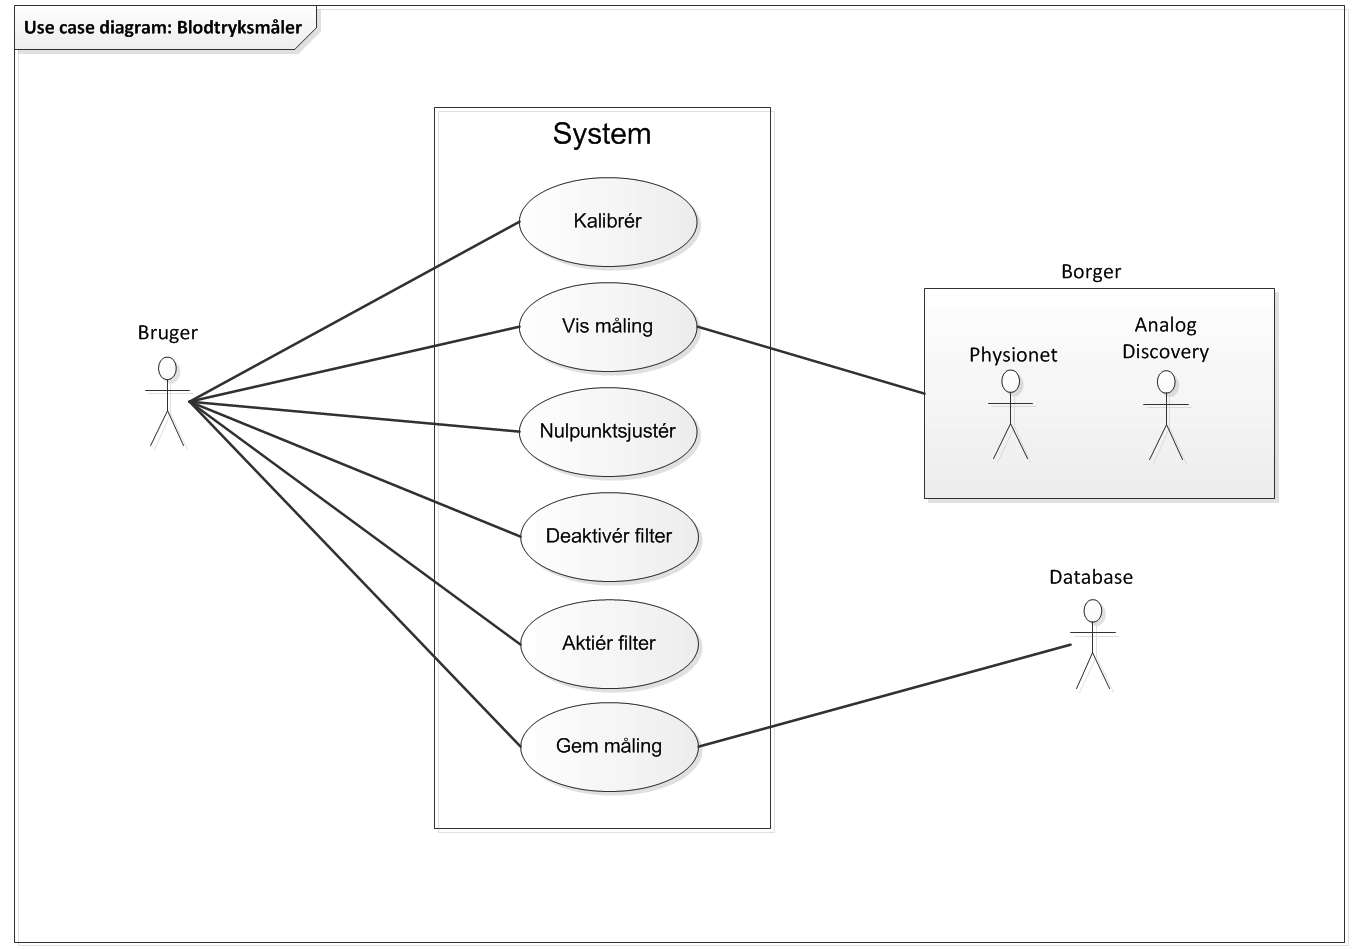
\includegraphics[width=1\textwidth]{Figurer/Snip20151001_20}
	\caption{Use case-diagram}
	\label{fig:Use case-diagram}
\end{figure}

Brugeren af systemet er den primære aktør i alle seks Use Cases. Det er Brugeren, der sætter alle Use Cases igang og styre, hvad der skal ske og hvornår. Borgeren, som er den sekundære aktør, integrer i UC2, da det er her, blodtryksmålingen for Borgeren skal vises. For at få gemt data integrer den sekundære aktør Database med UC6.  

\subsection{Use Cases}

\begin{longtabu} to \linewidth{@{}l r X[j]@{}} %UC1%
    {\large \textbf{Use Case 1}} && \\
    \toprule
    Navn &&    Kalibrér\\
    Use case ID &&    1\\
    Samtidige forløb &&    1\\
    Primær aktør &&    Bruger\\
    Sekundære aktør &&	 \\
    Mål &&    Bruger ønsker at kalibrere blodtrykssignal\\
    Initiering &&	Startes af Bruger\\
    Forudsætninger &&  System er aktivt og tilgængeligt\\
    Resultat &&		Blodtrykssignalet er kalibreret                         \\ \midrule
    Hovedforløb &    1. &	 Kalibrering-vinduet vises, hvor system spørger om der skal foretages en kalibrering\\[-1ex]  				
    			&    2. &    Bruger trykker på "Ja"\--knappen\newline
    						 [2.a \textit{Bruger trykker på "Nej"\--knappen}]\\
                &    3.	&	 System kalibrerer og Kalibrering-vinduet lukkes ned \newline\\ \midrule
                
    Undtagelser &    2.a &   Bruger ønsker ingen kalibrering. UC1 afsluttes og Kalibrering-vinduet lukkes  \\ \bottomrule
\caption{Fully dressed Use Case 1.}
\label{UC1}
\end{longtabu}


\begin{longtabu} to \linewidth{@{}l r X[j]@{}} %UC2%
    {\large \textbf{Use Case 2}} && \\
    \toprule
    Navn &&    Vis Måling\\
    Use case ID &&    2\\
    Samtidige forløb &&    1\\
    Primær aktør &&    Bruger\\
    Sekundære aktør &&	 Borger\\
    Mål &&    Bruger ønsker at vise blodtrykssignal med digitalt filter\\
    Initiering &&	Startes af UC1\\
    Forudsætninger &&  System er aktivt og tilgængeligt\\
    Resultat &&		Blodtrykssignalet udskrives                         \\ \midrule
    Hovedforløb &    1. &    Monitor-vinduet vises\\[-1ex]	
    			&    2. &    Blodtryksignal udskrives på en graf i 	  Monitor-vinduet\\[-1ex]
    			&	 3.	&	 Systole-, Diastole- og puls	værdier udskrives i Monitor-vinduet\newline\\ \midrule
                
    Undtagelser &    &   \\ \bottomrule
\caption{Fully dressed Use Case 2.}
\label{UC2}
\end{longtabu}


\begin{longtabu} to \linewidth{@{}l r X[j]@{}} %UC3%
    {\large \textbf{Use Case 3}} && \\
    \toprule
    Navn &&    Nulpunktsjustér\\
    Use case ID &&    3\\
    Samtidige forløb &&    1\\
    Primær aktør &&    Bruger\\
    Sekundære aktør && \\
    Mål &&    Bruger ønsker at nulpunktsjustere blodtrykssignal\\
    Initiering &&	Startes af Bruger\\
    Forudsætninger &&  System er aktivt og tilgængeligt. UC2 kører \\    Resultat &&		Blodtrykssignalet er nulpunktsjusteret\\ \midrule
    Hovedforløb &    1. &    Bruger trykker på "Nulpunktjustering"\--knappen\\[-1ex]   						 	
                &    2. &    System starter nulpunktsjusteringen\newline\\ \midrule
                
    Undtagelser &     &      \\ \bottomrule
\caption{Fully dressed Use Case 3.}
\label{UC3}
\end{longtabu}

\begin{longtabu} to \linewidth{@{}l r X[j]@{}} %UC4%
    {\large \textbf{Use Case 4}} && \\
    \toprule
    Navn &&    Deaktivér filter\\
    Use case ID &&    4\\
    Samtidige forløb &&   1\\
    Primær aktør &&    Bruger\\
    Sekundære aktør &&	 \\
    Mål &&    Bruger ønsker at deaktivere det digitale filter\\
    Initiering &&	Startes af Bruger\\
    Forudsætninger &&  System er aktivt og tilgængeligt. UC2 kører  \\
    Resultat &&		Ufiltreret blodtrykssignal vises i Monitor-vindet                 \\ \midrule
    Hovedforløb &    1. &    Bruger deaktiverer filter ved at markere i \textit{" Deaktivér digitalt filtre"} \\[-1ex]   						 	
                &    2. &    System udskriver det ufiltreret blodtryksignal\newline\\ \midrule
                
    Undtagelser &     &      \\ \bottomrule
\caption{Fully dressed Use Case 4.}
\label{UC4}
\end{longtabu}


\begin{longtabu} to \linewidth{@{}l r X[j]@{}} %UC5%
    {\large \textbf{Use Case 5}} && \\
    \toprule
    Navn &&    Aktivér filter\\
    Use case ID &&    5\\
    Samtidige forløb &&   1\\
    Primær aktør &&    Bruger\\
    Sekundære aktør &&	 \\
    Mål &&    Bruger ønsker at aktivere det digitale filter\\
    Initiering &&	Startes af Bruger\\
    Forudsætninger &&  System er aktivt og tilgængeligt. UC2 kører  \\
    Resultat &&		Filtreret blodtrykssignal vises i Monitor-vindet                 \\ \midrule
    Hovedforløb &    1. &    Bruger aktiverer filter ved at markere i \textit{" Aktivér digitalt filtre"} \\[-1ex]   						 	
                &    2. &    System udskriver det filtreret blodtryksignal\newline\\ \midrule
                
    Undtagelser &     &      \\ \bottomrule
\caption{Fully dressed Use Case 5.}
\label{UC5}
\end{longtabu}
    
\begin{longtabu} to \linewidth{@{}l r X[j]@{}} %UC6%
    {\large \textbf{Use Case 6}} && \\
    \toprule
    Navn &&    Gem måling\\
    Use case ID &&    6\\
    Samtidige forløb &&   *\\
    Primær aktør &&    Bruger\\
    Sekundære aktør &&	Database\\
    Mål &&    Bruger ønsker at gemme data i Database\\
    Initiering &&	Startes af Bruger\\
    Forudsætninger &&  System er aktivt og tilgængeligt. UC2 kører  \\
    Resultat &&		Data er gemt i Database                 \\ \midrule
    Hovedforløb &    1. &    Bruger trykker på "Gem"\--knappen \newline
       						 [1.a \textit{Borgerens data er gemt fra forrige målinger}]\\	
                &    2. &    System åbner Gem-vinduet\\[-1ex]
                &    3.	&	 Bruger indtaster data for blodtryksmålingen \\[-1ex]
                &	 4. &    Bruger trykker på "OK"\--knappen  \\[-1ex]
                &	 5.	&	 System lukker Gem-vinduet og åbner Monitor-vinduet igen\\[-1ex]
                &	 6.	&	 System viser, at data er gemt i Monitor-vinduet\newline
                
                \\ \midrule
                
    Undtagelser &   1.a  &  UC5 forsættes ved punkt 6    \\ \bottomrule
\caption{Fully dressed Use Case 6.}
\label{UC6}
\end{longtabu}


\section{Ikke-funktionelle krav}
De ikke-funktionelle krav er specificeret ved brug af redskabet (F)URPS+, der står for hhv. Functionality, Usability, Reliability, Performance, Supportability og andre krav til fx brugssituationer og interface.  


\subsection{Functionality}
\begin{itemize}
	\item System skal kunne vise en kontinuerlig blodtryksignal i Monitor-vinduet.
	\item System skal kunne vise Systole-, Diastole- og Pulsværdier med op til tre cifre.
	\item System skal kunne vise et blodtrykssignal med og uden et digitalt filter.
	\item System skal kunne nulpunktsjustere blodtrykssignalet.
	\item System skal kunne gemme en blodtryksmåling i en database.
	\item System skal kunne kalibreres. 
\end{itemize}

\subsection{Usability}
\begin{itemize}
	\item Monitor-vinduet skal indeholde en ”Gem”\--knap.
	\item Monitor-vinduet skal indeholde en ”Nulpunktsjustér”\--knap.
	\item Monitor-vinduet skal indeholde to radiobuttons til aktivering og deaktivering af digitalt filter.
	\item Kalibrering-vinduet skal indeholde en ”Ja”\--knap og en ”Nej”\--knap.
	\item Kalibrering-vinduet skal indeholde et datostempel for seneste kalibrering.
	\item Gem-vinduet skal indeholde tekstbokse til data indtastning for målingen. 
	\item Gem-vinduet skal indeholde en ”OK”\--knap.
	\item Det skal være muligt at aflæse værdier på Monitor-vinduet fra 2 meters afstand med normalt syn.
\end{itemize}

\subsection{Reliability}
\begin{itemize}
	\item Systemet skal have en effektiv MTBF (Mean Time Between Failure) på 20 minutter og en MTTR (Mean Time To Restore) på 1 minut.
				\begin{align}
					Availability = \frac{MTBF}{MTBF+MTTR} = \frac{20}{20+1} = 0,952 = 95,2 \%
				\end{align}

\end{itemize}

\subsection{Performance}
\begin{itemize}
	\item Blodtrykssignalet skal vises maksimalt 5 sekunder efter UC1 er afsluttet.
	\item Systemet skal vise en graf for blodtryksmålingen, hvor y-aksen er mmHg og x-aksen er tid i sekunder.
	\item Systemet skal kunne måle blodtryksværdier fra 0 til 300 mmHg.
\end{itemize}

\subsection{Supportability}
\begin{itemize}
	\item Softwaren skal opbygges efter trelagsmodellen.
\end{itemize}

\subsection{Andre(+)}
\textbf{Brugssituationer}
\begin{itemize}
	\item Der skal være adgang til en computer med Windows 7 eller nyere – computeren skal have minimum 4 GB RAM.
\end{itemize}
\textbf{Interface}
\begin{itemize}
	\item Blodtryksdiagrammet skal fylde minimum 1/3 af Monitor-vinduet.
	\item Baggrunden i Montior-vinduet skal være mørk.
	\item Blodtrykssignal og -værdier(systole og diastole) skal være røde, og puls skal være grøn.
	\item Systolisk og diastolisk blodtryk skal fremhæves ved større skriftstørrelse end andre værdier i Monitor-vinduet (fx værdier på akserne).
\end{itemize}













